\documentclass[a4paper,10pt,oneside]{article}
\usepackage[polutonikogreek,italian]{babel}
\usepackage[utf8x]{inputenc}
\usepackage{amsmath}
\usepackage{amsthm}
\usepackage{amssymb}
\usepackage{amscd}
\usepackage{graphicx}
\usepackage{float}
\usepackage{array}
\usepackage{rotating}
\usepackage[small]{caption}
\usepackage{lscape}
\usepackage{fancybox}
\usepackage{booktabs}
\usepackage[noanswer]{exercise}
\parindent0ex
\renewcommand{\fboxsep}{0.4cm}
\usepackage{hyperref}
\renewcommand{\textfraction}{0.05}
\renewcommand{\topfraction}{0.95}
\renewcommand{\bottomfraction}{0.95}
\renewcommand{\floatpagefraction}{0.35}
\renewcommand{\ExerciseName}{Esercizio}
\renewcommand{\ExerciseListName}{Es}
\setcounter{totalnumber}{5}
\restylefloat{figure}
\begin{document}

\section*{Misura accelerazione}

\subsection*{Utilizzando due misure di tempo}

Posiziono il primo rilevatore in modo che il carrello lambisca il fotodiodo. Al tempo $t=0$ il carrello viene lasciato libero e il primo contatore parte 

\begin{figure}[H]
 \centering
 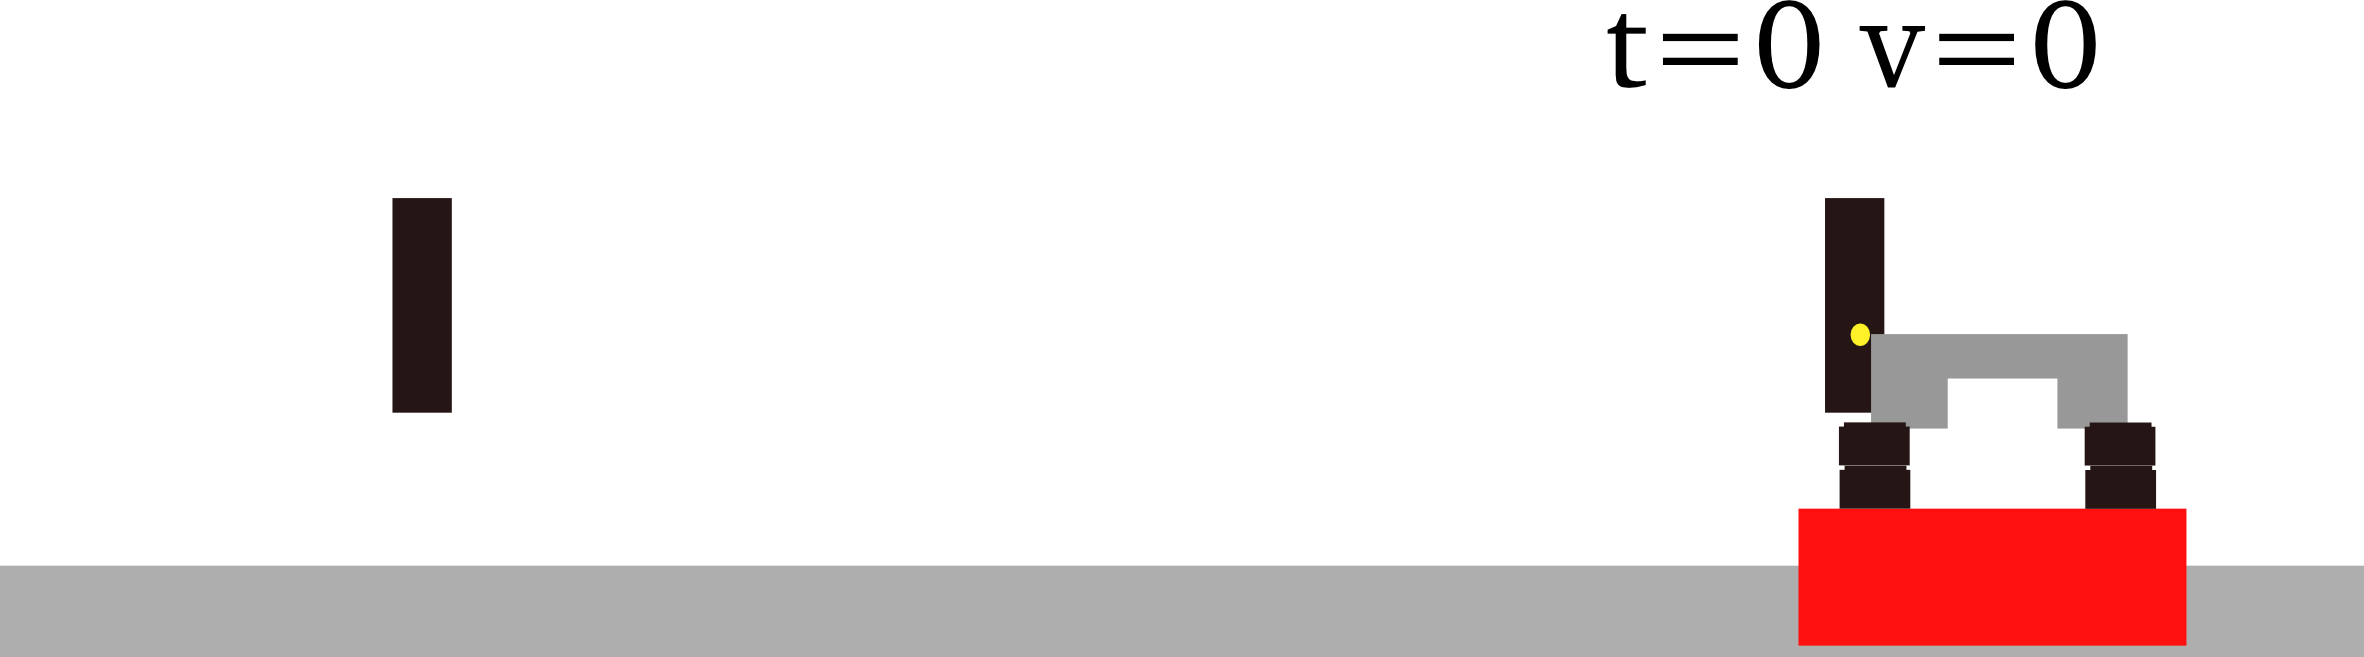
\includegraphics[width=\textwidth]{./immagini/misura_accelerazione1.png}
 % misura_accelerazione1.png: 2364x657 pixel, 288dpi, 20.89x5.80 cm, bb=0 0 592 165
 \label{fig:accelerazione1}
\end{figure}

il carrello si muove con accelerazione uniforme fino a lambire il fotodiodo del secondo rilevatore al tempo $t=T$ con velocità $v=v_1$ il cronometro registra il tempo $T$. Il cronometro inizia a misurare il tempo di transito del carrello attraverso il secondo rilevatore

\begin{figure}[H]
 \centering
 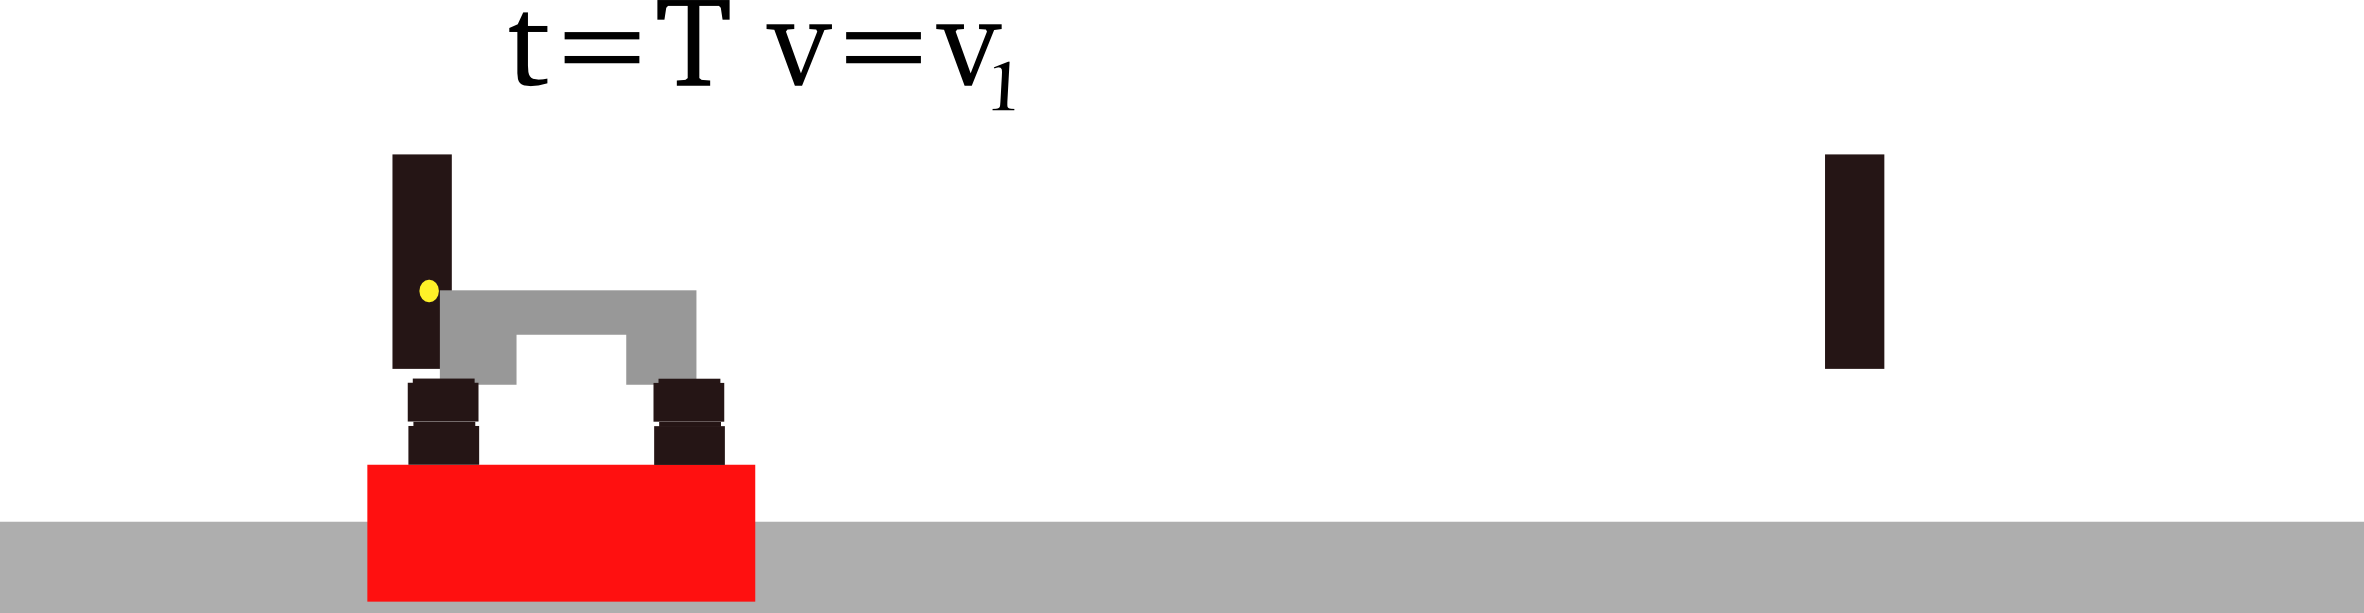
\includegraphics[width=\textwidth]{./immagini/misura_accelerazione2.png}
 % misura_accelerazione2.png: 2364x613 pixel, 288dpi, 20.89x5.42 cm, bb=0 0 592 154
 \label{fig:accelerazione2}
\end{figure}

il carrello è appena transitato oltre il secondo rilevatore il tempo è  $t=T+\Delta t$ la velocità $v=v_2$ Il cronometro misura il tempo $\Delta t$.
\begin{figure}[H]
 \centering
 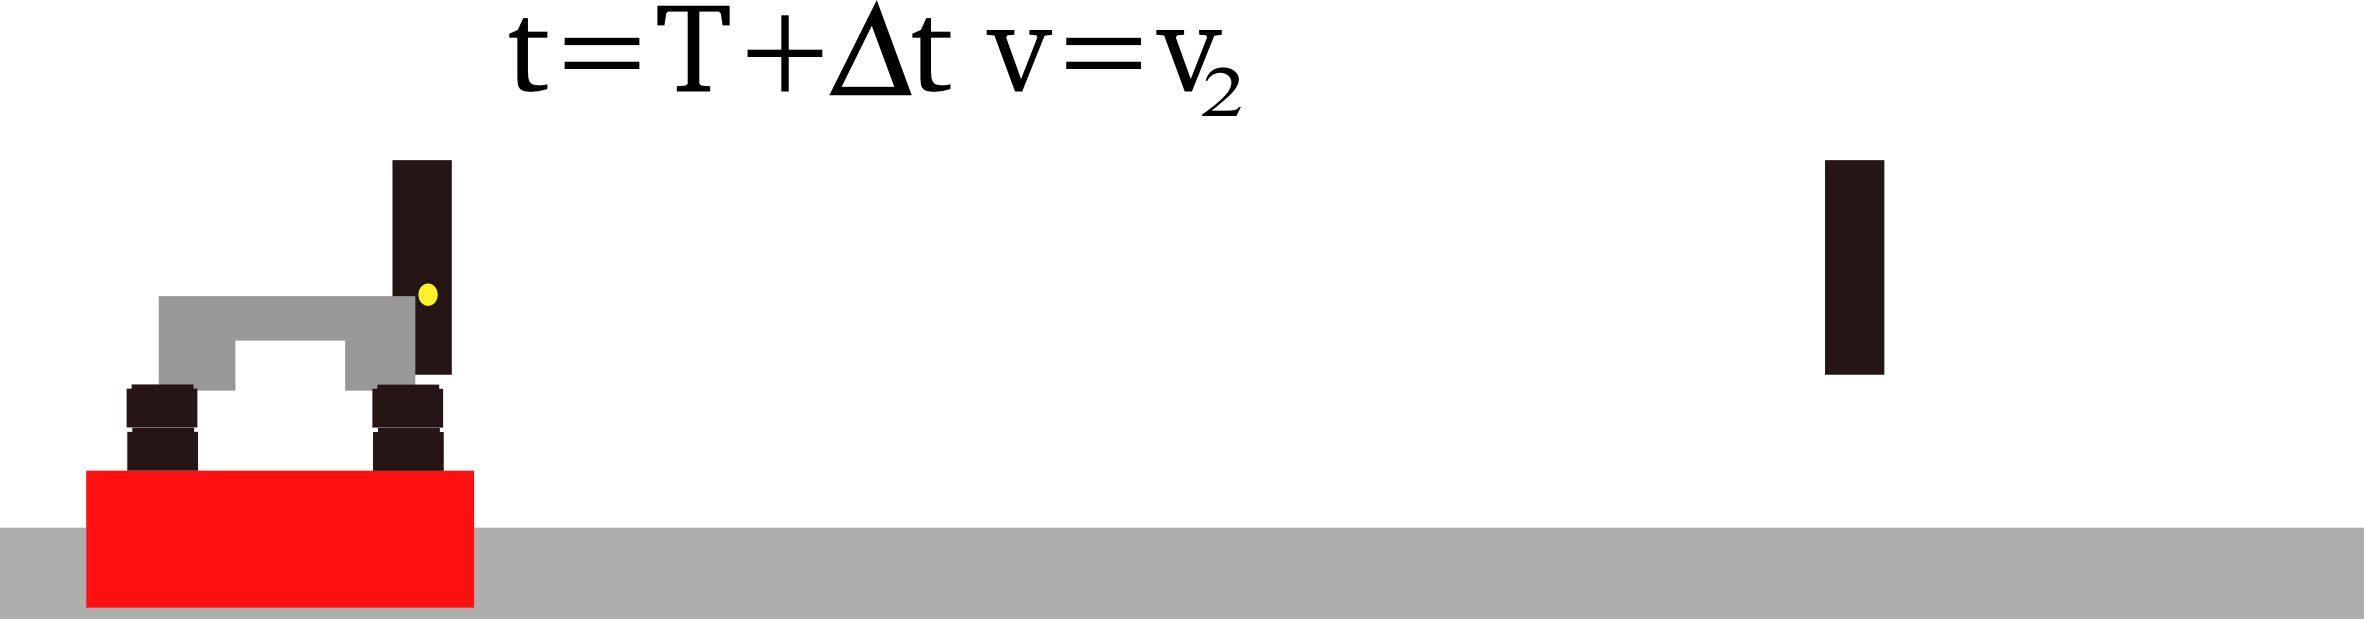
\includegraphics[width=\textwidth]{./immagini/misura_accelerazione3.png}
 % misura_accelerazione3.png: 2364x619 pixel, 288dpi, 20.89x5.47 cm, bb=0 0 592 155
 \label{fig:accelerazione3}
\end{figure}

Siccome il moto è uniformemente accelerato se chiamo $L$ la lunghezza del vagone posso dire che la media delle velocità $v_1$ e $v_2$ sarà uguale alla velocità media di transito del carrello quindi:
\begin{equation}
 \frac 1 2(v_1+v_2)=\frac{L}{\Delta t}
\end{equation}

come abbiamo detto oggi in laboratorio l'istante di tempo in cui la velocità è pari alla velocità media è $t=T+\Delta t/2$  per cui la variazione di velocità del carrello nel tempo $T+\Delta t/2$ è pari a:
\begin{equation}
 \Delta v=\frac{L}{\Delta t}
\end{equation}

e l'accelerazione è quindi:
\begin{equation}
 a=\frac{2L}{\Delta t(2T+\Delta t)}
\end{equation}


\subsection*{Utilizzando una misura di tempo e una di spazio}

Significato dei simboli:
\begin{itemize}
 \item $v_0=0$ velocità iniziale
 \item $v_1$ velocità nell'istante in cui la parte anteriore della banderuola oltrepassa la fotocellula
 \item $v_2$ velocità nell'istante in cui la parte posteriore della banderuola oltrepassa la fotocellula
\item $\Delta t$ tempo impiegato dalla banderuola per oltrepassare la fotocellula
\item $L$ lunghezza della banderuola
\item $s$ distanza tra la parte anteriore della banderuola e la fotocellula al tempo $t=0$
\item $a$ accelerazione incognita
\end{itemize}

I valori misurati sono $\Delta t$, $L$ ed $s$, con le notazioni sopra esposte possiamo scrivere:
\begin{equation}
 \begin{cases}
    v_1^2=2as\\
    v_2=v_1+a\Delta t\\
    \frac 1 2(v_1+v_2)=\frac{L}{\Delta t}
 \end{cases}
\end{equation}
da cui otteniamo un'equazione per l'accelerazione:
\begin{equation}
 \frac{1}{2}a\Delta t+\sqrt{2s}\sqrt{a}-\frac{L}{\Delta t}=0
\end{equation}

la cui soluzione ci da l'accelerazione:
\begin{equation}
 a=\frac{2(L+2s-2\sqrt{s(L+s}))}{\Delta t^2}
\end{equation}



\end{document}
